%% fig_twohalves.tex   (generated by make_round28.py; do not edit by hand)
%% The two halves of the conjecture in thm:final: a Hodge class on X is carried by an algebraic correspondence from a Hodge class on an abelian variety (F3'), which is algebraic (F2); the Weil families are the plate where thm:main applies.
\documentclass[tikz,border=8pt]{standalone}
\usepackage{amsmath,amssymb}
\usetikzlibrary{arrows.meta,calc,decorations.pathreplacing}
%% palette.tex -- shared colour definitions for the figures
\definecolor{PInk}{RGB}{26,32,44}
\definecolor{PBlue}{RGB}{37,82,139}
\definecolor{PTeal}{RGB}{23,127,125}
\definecolor{POchre}{RGB}{193,138,44}
\definecolor{PClay}{RGB}{178,74,58}
\definecolor{PSlate}{RGB}{108,122,137}
\definecolor{PViolet}{RGB}{110,86,150}
\definecolor{WBlue}{RGB}{223,234,246}
\definecolor{WTeal}{RGB}{220,238,236}
\definecolor{WOchre}{RGB}{250,240,218}
\definecolor{WClay}{RGB}{247,229,224}
\definecolor{WSlate}{RGB}{238,241,244}
\definecolor{PMag}{RGB}{158,58,110}
\definecolor{PGrass}{RGB}{62,124,66}
\definecolor{PAmber}{RGB}{214,112,38}
\definecolor{PIndigo}{RGB}{58,64,140}
\definecolor{PRule}{RGB}{176,186,197}

%% shared macros so the standalone figures match the paper
\providecommand{\QQ}{\mathbb{Q}}
\providecommand{\ZZ}{\mathbb{Z}}
\providecommand{\RR}{\mathbb{R}}
\providecommand{\CC}{\mathbb{C}}
\providecommand{\PP}{\mathbb{P}}
\providecommand{\Kx}{K^{\times}}
\providecommand{\HW}{W}
\providecommand{\Nm}{\mathrm{N}}
\providecommand{\Hdg}{\mathrm{Hdg}}
\providecommand{\NS}{\mathrm{NS}}
\providecommand{\cA}{\mathcal{A}}
\providecommand{\cD}{\mathcal{D}}
\providecommand{\cF}{\mathcal{F}}
\providecommand{\cP}{\mathcal{P}}
\providecommand{\cO}{\mathcal{O}}
\providecommand{\cQ}{\mathcal{Q}}
\providecommand{\bbar}[1]{\overline{#1}}
\providecommand{\ch}{\operatorname{ch}}
\providecommand{\End}{\mathrm{End}}
\providecommand{\Ext}{\operatorname{Ext}}
\providecommand{\Supp}{\operatorname{Supp}}

\begin{document}
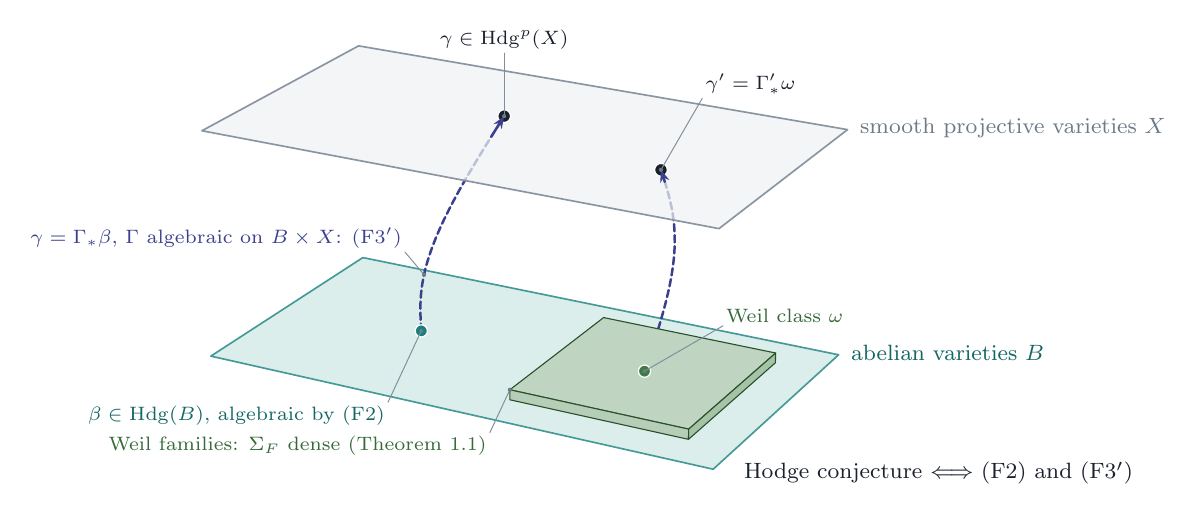
\begin{tikzpicture}[x=1cm,y=1cm,line join=round,line cap=round,
  font=\small,text=PInk,lbl/.style={inner sep=1pt}]
  \path[fill=WTeal,draw=PTeal!80,line width=0.60pt] (-3.9881,-1.2601) -- (2.3910,-2.6962) -- (3.9843,-1.2432) -- (-2.0574,-0.0086) -- cycle;
  \draw[PIndigo,line width=0.9pt,dash pattern=on 2.6pt off 1.4pt] (-1.3156,-0.9395) -- (-1.3185,-0.8935) -- (-1.3213,-0.8472) -- (-1.3237,-0.8005) -- (-1.3256,-0.7532) -- (-1.3268,-0.7052) -- (-1.3272,-0.6565) -- (-1.3266,-0.6069) -- (-1.3247,-0.5562) -- (-1.3215,-0.5045) -- (-1.3169,-0.4515) -- (-1.3106,-0.3973) -- (-1.3025,-0.3418) -- (-1.2926,-0.2848) -- (-1.2807,-0.2263) -- (-1.2668,-0.1663) -- (-1.2507,-0.1047) -- (-1.2323,-0.0414) -- (-1.2117,0.0234) -- (-1.1888,0.0899) -- (-1.1636,0.1581) -- (-1.1361,0.2279) -- (-1.1062,0.2993) -- (-1.0740,0.3723) -- (-1.0396,0.4469) -- (-1.0029,0.5229) -- (-0.9641,0.6004) -- (-0.9233,0.6793) -- (-0.8805,0.7595) -- (-0.8359,0.8409) -- (-0.7895,0.9234) -- (-0.7415,1.0069) -- (-0.6921,1.0914) -- (-0.6413,1.1767) -- (-0.5894,1.2627) -- (-0.5365,1.3494) -- (-0.4828,1.4365) -- (-0.4284,1.5240) -- (-0.3735,1.6119) -- (-0.3183,1.6998);
  \draw[PIndigo,line width=0.9pt,dash pattern=on 2.6pt off 1.4pt] (1.5190,-1.4510) -- (1.5453,-1.3722) -- (1.5716,-1.2935) -- (1.5975,-1.2150) -- (1.6231,-1.1369) -- (1.6482,-1.0591) -- (1.6726,-0.9818) -- (1.6963,-0.9051) -- (1.7192,-0.8291) -- (1.7410,-0.7538) -- (1.7618,-0.6793) -- (1.7815,-0.6057) -- (1.7999,-0.5330) -- (1.8169,-0.4614) -- (1.8326,-0.3907) -- (1.8468,-0.3212) -- (1.8595,-0.2527) -- (1.8707,-0.1854) -- (1.8802,-0.1192) -- (1.8881,-0.0542) -- (1.8944,0.0097) -- (1.8990,0.0725) -- (1.9020,0.1341) -- (1.9033,0.1946) -- (1.9030,0.2540) -- (1.9011,0.3124) -- (1.8977,0.3698) -- (1.8928,0.4263) -- (1.8864,0.4819) -- (1.8786,0.5366) -- (1.8696,0.5905) -- (1.8593,0.6438) -- (1.8478,0.6965) -- (1.8354,0.7486) -- (1.8219,0.8003) -- (1.8077,0.8516) -- (1.7928,0.9026) -- (1.7772,0.9535) -- (1.7612,1.0043) -- (1.7449,1.0551);
  \fill[PTeal,draw=white,line width=0.45pt] (-1.3156,-0.9395) circle (2.20pt);
  \path[fill=PGrass!33!white,draw=PGrass!65!black,line width=0.40pt] (-0.1910,-1.6875) -- (2.0805,-2.1872) -- (3.1852,-1.2206) -- (0.9999,-0.7705) -- cycle;
  \path[fill=PGrass!38!white,draw=PGrass!65!black,line width=0.40pt] (-0.1907,-1.8145) -- (2.0778,-2.3169) -- (2.0805,-2.1872) -- (-0.1910,-1.6875) -- cycle;
  \path[fill=PGrass!46!white,draw=PGrass!65!black,line width=0.40pt] (2.0778,-2.3169) -- (3.1812,-1.3449) -- (3.1852,-1.2206) -- (2.0805,-2.1872) -- cycle;
  \fill[PGrass,draw=white,line width=0.45pt] (1.5190,-1.4510) circle (2.20pt);
  \path[fill opacity=0.72,fill=WSlate,draw=PSlate!80,line width=0.60pt] (-4.1020,1.6019) -- (2.4650,0.3591) -- (4.0980,1.6165) -- (-2.1119,2.6803) -- cycle;
  \fill[PInk,draw=white,line width=0.45pt] (-0.2629,1.7879) circle (2.30pt);
  \fill[PInk,draw=white,line width=0.45pt] (1.7283,1.1060) circle (2.30pt);
  \draw[PIndigo,line width=0.9pt,-{Stealth[length=4.4pt,width=3.4pt]}] (-0.4284,1.5240) -- (-0.3735,1.6119) -- (-0.3183,1.6998) -- (-0.2629,1.7879);
  \draw[PIndigo,line width=0.9pt,-{Stealth[length=4.4pt,width=3.4pt]}] (1.7772,0.9535) -- (1.7612,1.0043) -- (1.7449,1.0551) -- (1.7283,1.1060);
  \draw[PSlate!85,line width=0.35pt] (-0.2629,2.5879) -- (-0.2629,1.7879);
  \fill[PSlate] (-0.2629,1.7879) circle (0.75pt);
  \draw[PSlate!85,line width=0.35pt] (2.2533,2.0153) -- (1.7283,1.1060);
  \fill[PSlate] (1.7283,1.1060) circle (0.75pt);
  \draw[PSlate!85,line width=0.35pt] (-1.7382,-1.8458) -- (-1.3156,-0.9395);
  \fill[PSlate] (-1.3156,-0.9395) circle (0.75pt);
  \draw[PSlate!85,line width=0.35pt] (-0.4445,-2.2313) -- (-0.1910,-1.6875);
  \fill[PSlate] (-0.1910,-1.6875) circle (0.75pt);
  \draw[PSlate!85,line width=0.35pt] (2.5149,-0.8760) -- (1.5190,-1.4510);
  \fill[PSlate] (1.5190,-1.4510) circle (0.75pt);
  \draw[PSlate!85,line width=0.35pt] (-1.5218,0.0610) -- (-1.2807,-0.2263);
  \fill[PSlate] (-1.2807,-0.2263) circle (0.75pt);
  \node[lbl,anchor=west,text=PSlate,font=\footnotesize] at (4.2162,1.6373) {smooth projective varieties $X$};
  \node[lbl,anchor=west,text=PTeal!80!black,font=\footnotesize] at (4.1025,-1.2224) {abelian varieties $B$};
  \node[lbl,anchor=south,text=PInk,font=\scriptsize] at (-0.2629,2.5879) {$\gamma\in\Hdg^{p}(X)$};
  \node[lbl,anchor=west,text=PInk,font=\scriptsize] at (2.2533,2.1945) {$\gamma'=\Gamma'_{*}\omega$};
  \node[lbl,anchor=east,text=PTeal!80!black,font=\scriptsize] at (-1.7382,-2.0110) {$\beta\in\Hdg(B)$, algebraic by (F2)};
  \node[lbl,anchor=east,text=PGrass!85!black,font=\scriptsize] at (-0.4445,-2.3965) {Weil families: $\Sigma_{F}$ dense (\textup{Theorem 1.1})};
  \node[lbl,anchor=west,text=PGrass!85!black,font=\scriptsize] at (2.5149,-0.7484) {Weil class $\omega$};
  \node[lbl,anchor=east,text=PIndigo,font=\scriptsize] at (-1.5218,0.2358) {$\gamma=\Gamma_{*}\beta$, $\Gamma$ algebraic on $B\times X$: (F3$'$)};
  \node[lbl,anchor=west,text=PInk,font=\footnotesize] at (2.7410,-2.7462) {Hodge conjecture $\Longleftrightarrow$ (F2) and (F3$'$)};
\end{tikzpicture}
\end{document}
